PAMELA is composed of one design time component (the PAMELA metamodel, plus a number of predefined annotations) presented in the next section and one runtime component (the PAMELA interpreter), described in Section \ref{sub:RunTime}.

%\subsection{Installation}
%\label{sub:installation}

%\todo{Maybe a word on how to install.}
% We decided not to do it

\begin{center}
\begin{figure}
    %\centering
    %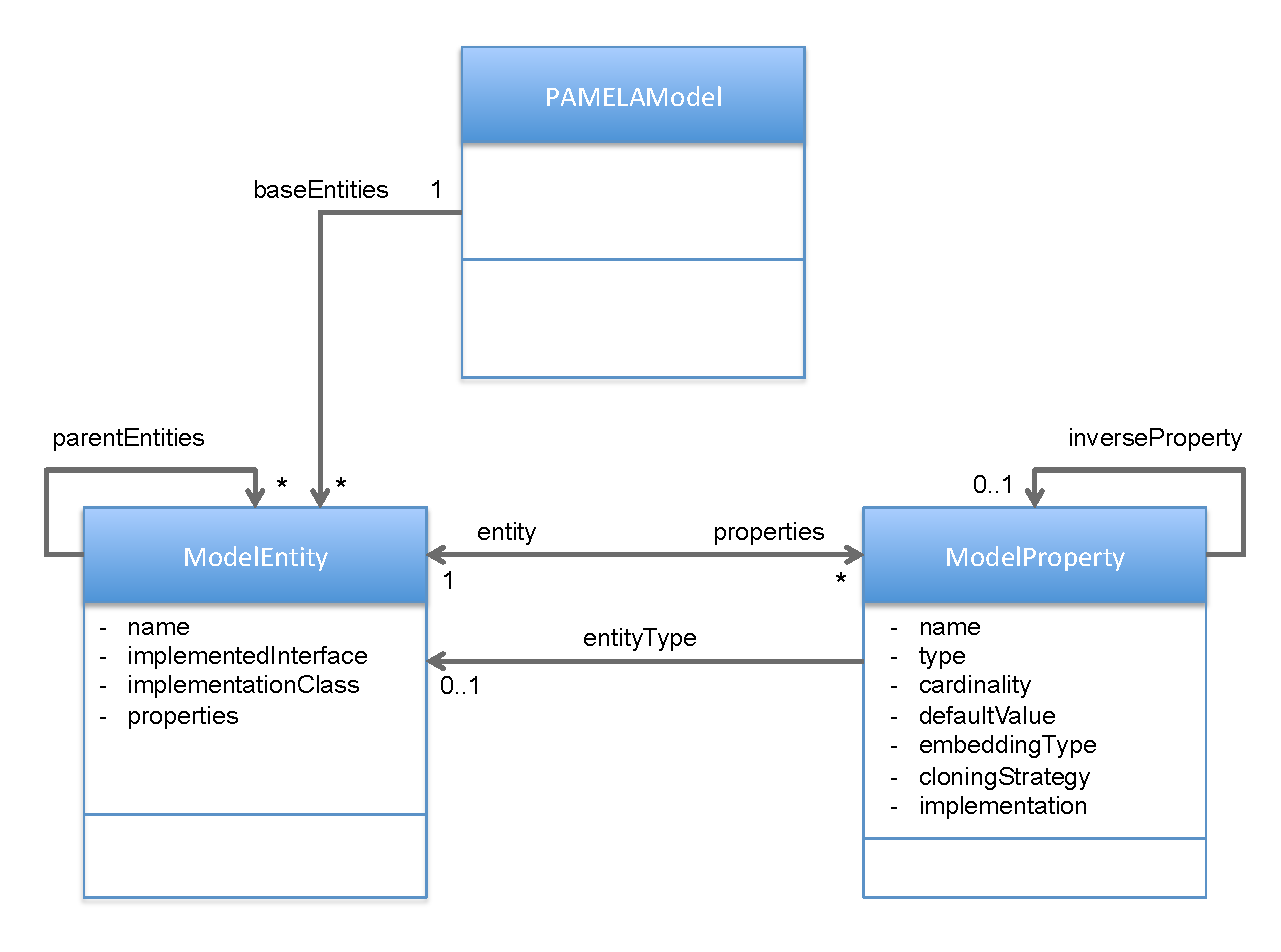
\includegraphics[width=1.0 \columnwidth]{PamelaMetaModel.pdf}
    \begin{tikzpicture}[scale=0.9]
    \useasboundingbox (-9,-5) rectangle (3,0);% ajustement à la main :-(
    \umlclass[x=-2,y=0]{PAMELAModel}{}{}
    \umlclass[x=-6,y=-3]{ModelEntity}{-- name \\ -- implementationInterface \\ -- implementationClass}{}
    \umlclass[x=2,y=-3]{ModelProperty}{-- name \\ -- type \\ -- cardinality \\ -- defaultValue \\ -- embeddingType \\ -- cloningStrategy \\ -- implementation }{}
    \umluniassoc[geometry=-|, arg1=baseEntities, mult1=1, pos1=0.45,  arg2=*, pos2=1.9]{PAMELAModel}{ModelEntity}
    \umluniassoc[arg1=entity, pos1=0.15, mult1=1, anchors=20 and 154, arg2=properties, mult2=*, pos2=0.75]{ModelEntity}{ModelProperty}
    \umluniassoc[anchors=154 and 20]{ModelProperty}{ModelEntity}
    \umluniassoc[mult1=entityType, pos1=0.5, arg2=0..1, pos2=0.9]{ModelProperty}{ModelEntity}
    \umluniassoc [arg=parentEntities , mult=*, pos=0.9, align= right, angle1=170, angle2=110, loopsize=2cm]{ModelEntity}{ModelEntity}
    \umluniassoc [arg=inverseProperty , mult=0..1, pos=0.9, align= left, angle1=20, angle2=80, loopsize=2cm]{ModelProperty}{ModelProperty}
    \end{tikzpicture}
    \caption{PAMELA metamodel}
    \label{fig:PamelaMetaModel}
\end{figure}
\end{center}
    
\subsection{Design time}
\label{sub:DesignTime}

The PAMELA metamodel is depicted in Figure~\ref{fig:PamelaMetaModel}, and allows, through the use of annotations, the definition of \emph{simple} UML-like models directly on the code.

A \texttt{PAMELAModel} is defined as a set of references to \texttt{ModelEntity}. A \texttt{Model\-Entity} reflects a concept and is encoded in a Java \texttt{interface}. 
Then, a \texttt{Model\-Entity} only defines an API (Application Programming Interface) without any implementation for methods. 
Note that \emph{ModelEntities} may declare \emph{ImplementationClasses}, which
will be responsible for providing custom code implementing domain or
application-specific behavior. A partially implemented \texttt{abstract} Java
\texttt{class} may be defined as partial base implementation (conforms to
implemented interface), as default methods in Java interfaces would be
(since Java 8).
The PAMELA metamodel allows multiple inheritance: thus \texttt{ModelEntity} may define a set of parent entities. 

A \texttt{ModelEntity} also defines some properties, encoded as \texttt{ModelProperty}. A \texttt{ModelProperty} is identified by a name, a cardinality (simple or multiple) and a type, which can be a reference to another \texttt{ModelEntity}, or a Java type (a primitive or an arbitrary complex Java type). Depending on its cardinality, a \texttt{ModelProperty} is bound to a set of methods reflecting use of property.
\begin{itemize}
    \item A \emph{read-only single property} will define read access of its value using a \emph{getter} (a Java method defined in Java interface taking no argument and returning the desired value).
    \item A \emph{read-write single property} will define a \emph{getter} and a \emph{setter} (a Java method taking the value to be set as unique argument).
    \item A \emph{read-write multiple property} will define a \emph{getter}, an \emph{adder} (a Java method taking the value to be added as unique argument), a \emph{remover} (a Java method taking the value to be removed as unique argument), and may define additional methods for extended features such as re-indexing, for example.
\end{itemize}


In the following we list the most common Java annotations used in the context of \texttt{ModelEntity} and \texttt{ModelProperty} definitions:

\begin{itemize}
    \item \texttt{@ModelEntity}: tag annotating \texttt{interface} as \emph{ModelEntity}. May also declare an abstract entity.
    \item \texttt{@ImplementationClass}: tag annotating \emph{ModelEntity} \texttt{interface} and precising abstract Java \texttt{class} to be used as base implementation.
    \item \texttt{@Implementation}: tag annotating a partial implementation (abstract inner \texttt{class} defined in implemented \texttt{interface}), and used in the context of multiple inheritance.
    \item \texttt{@Getter(String)}: tag annotating method as unique getter for implicit \emph{ModelProperty} whose identifier is the declared String value. May also declares cardinality, eventual inverse property, default value and some other features.
    \item \texttt{@Setter(String)}: tag annotating method as unique setter for implicit \emph{ModelProperty} whose identifier is the declared String value.
    \item \texttt{@Adder(String)}: tag annotating method as unique adder for implicit multiple cardinality \emph{ModelProperty} whose identifier is the declared String value.
    \item \texttt{@Remover(String)}: tag annotating method as unique remover for implicit multiple cardinality \emph{ModelProperty} whose identifier is the declared String value.
    \item \texttt{@Reindexer(String)}: tag annotating method as unique re-indexer for implicit multiple cardinality \emph{ModelProperty} whose identifier is the declared String value.
    \item \texttt{@Initializer}: tag annotating a method used as a constructor for related \emph{ModelEntity}.
   \item \texttt{@Deleter}: tag annotating a method used as explicit destructor for related \emph{ModelEntity}.
    \item \texttt{@Finder(String,String)}: tag annotating method as a fetching request for a given \emph{ModelProperty} with a given attribute.
    \item \texttt{@CloningStrategy}: allows to customize cloning strategy for a given \emph{ModelProperty}.
    \item \texttt{@Embedded}: allows to declare a given \emph{ModelProperty} as
      embedded. %according to PAMELA semantics.
    \item \texttt{@Imports} and \texttt{@Imports}: allows to declare some entities to be included in PAMELA model.
    \item \texttt{@XMLElement} and \texttt{@XMLAttribute}: used to specify XML serialization for PAMELA instances.
    
\end{itemize}

 \subsection{Runtime}
 \label{sub:RunTime}
 
 The aforementioned models are executed at runtime as a combination of two components as illustrated by  the right part of Figure~\ref{fig:PamelaVision}: 1) plain Java bytecode, as the result of the basic compilation of source code; and 2) an embedded PAMELA interpreter, executing semantics reflected by \emph{ModelEntity} and \emph{ModelProperty}  declarations (together with custom annotations where available).

The main idea for the approach is to override Java dynamic binding. Invoking a method on an object which is part of a PAMELA model, causes the real implementation to be called when existing (more precisely dispatch code execution between all provided implementations), or the required interpretation according to the underlying model to be executed. 
 
The PAMELA interpreter will intercept any method call for all instances of \emph{ModelEntity} and conditionally branches code execution.
 \begin{itemize}
     \item If the accessed method is part of a \emph{ModelProperty} (a getter, or a setter, etc.), and no custom implementation is defined neither in the class declared as implementation, nor in a class declared as partial implementation in the context of traits, then, execution is delegated to the related property implementation (generic code provided by the PAMELA interpreter).
     \item If the accessed method is defined in a class declared as implementation, or in a class declared as partial implementation, then this method is executed. The PAMELA API through the \mytexttt{AccessibleProxyObject} interface also provides access to generic behavior (super implementation), allowing the developer to define an overriding composition.
 \end{itemize}
 
This general scheme also provides an extension point allowing to instrument the code. This extension point is used in order to integrate other features such as notification management, undo/redo stack management, assertion checking at runtime (support for \emph{Design by Contract}, aka JML), and dynamic code weaving in the context of \emph{Aspect Programming}.

The PAMELA model at runtime is computed dynamically, working on the classpath of
launched Java application, and starting from a simple Java interface (or a
collection of Java interfaces) which is/are PAMELA-annotated. From a
mathematical point of view, internal representation of the underlying model is
a graph whose vertices are PAMELA \emph{ModelEntities} (annotated Java
interface), and edges are either inheritance links or reference links (a
property whose type is another \emph{ModelEntity}). \mytexttt{@Imports} and
  \mytexttt{@Import} annotations allow to include some other
  \emph{ModelEntities} in the model. An annotation attribute
  \mytexttt{@Getter(...ignoreType=true)} allows to ignore the link. In that
  context, PAMELA model computation is a graph closure computation, starting
  from a collection of vertices.

%\footnote{Model closure computation on-the-fly provides an interesting approach to deal with model fragmentation.} 
A PAMELA model at runtime is represented by a \mytexttt{ModelContext}.

PAMELA instances (instances of \emph{ModelEntity}) are handled through the use of \mytexttt{ModelFactory}, which is instantiated from a \mytexttt{ModelContext}.

% Folloging section/itemize may be removed when needed 
%This composition offers many benefits: 
%\begin{itemize}
%    \item Strong coupling between model and code
%    \item Strong typing is kept, and required checks are performed by the Java compiler
%    \item PAMELA framework provides interpretation of model@runtime
%    \item No need to generate POJO (Plain Old Java Objects), as their
%    execution follow the standard semantics (less code, fewer bugs)
%    \item Custom implementation are provided if needed, using classical Java extension points
%    \item It offers a way to intercept method calls and instrument the code
%    \item Assertions checking at runtime
%    \item Dynamic code weaving at runtime (aspect programming without compilation)
%\end{itemize}

\subsection{Additional Features}

Programmers may already reuse a number of advanced programming features
(some already mentioned) such as: multiple inheritance and traits, containment
management, cloning, fine-grained notification management, object graph
comparison and diff/merge, visiting patterns, clipboard management, validation,
support for \emph{design by contract} by integrating assertions from Java
Modeling Language (JML), Metaprogramming, Aspect Oriented Programming. Each of
those features is described on a dedicated page that is reachable from the
official web site\footnote{\url{https://pamela.openflexo.org}}.
Experimented programmers may extend PAMELA defining new annotations.

%A strong interest of the approach is that the model is encoded in Java, and must be compiled. It forces the Java compiler to perform required checks %for a PAMELA model encoded in a strong typed program. Execution semantics of model is fully compatible with Java semantics. Many validation rules %are automatically performed through classical Java compilation, independently of underlying PAMELA execution semantics.

\subsection{Example}

Listing \ref{lst:model} shows a very basic model with two entities: \emph{Book} and \emph{Library}. Entity \emph{Book} defines two read-write single properties (\emph{title} and \emph{ISBN}) with single cardinality and with \texttt{String} type. Entity \emph{Book} also defines a constructor with initial \emph{title} value. Entity \emph{Library} defines a read-write multiple properties \emph{books} referencing \emph{Book} instances. Note that this code is sufficient to execute the model, while no additional line of code is required (only Java interfaces and API methods are declared here). 

%\begin{figure}
%    \centering
\begin{lstlisting}[language=Java,basicstyle=\ttfamily\footnotesize, caption=Model creation, label=lst:model]
@ModelEntity
public interface Book extends AccessibleProxyObject {

  @Initializer
  public Book init(@Parameter("title")String aTitle);
  
  @Getter("title")
  public String getTitle();
  
  @Setter("title")
  public void setTitle(String aTitle);
  
  @Getter("ISBN")
  public String getISBN();
  
  @Setter("ISBN")
  public void setISBN(String value);
}

@ModelEntity
public interface Library extends AccessibleProxyObject {

  @Getter(value = "books", cardinality = Cardinality.LIST)
  public List<Book> getBooks();

  @Adder("books")
  public void addToBooks(Book aBook);

  @Remover("books")
  public void removeFromBooks(Book aBook);

  @Reindexer("books")
  public void moveBookToIndex(Book aBook, int index);
  
  @Finder(collection = "books", attribute = "title")
  public Book getBook(String title);
}
\end{lstlisting}
 %   \caption{A basic PAMELA model with two entities \texttt{Library} and \texttt{Book}}
 %   \label{fig:ABasicPamelaModel}
%\end{figure}

The execution and the management of this model may be performed using the following simple lines of code:

%\begin{figure}
%    \centering
\begin{lstlisting}[language=Java,basicstyle=\ttfamily\footnotesize, caption=model execution/manipulation, label=lst:execution]
// Instantiate the meta-model
// by computing the closure of concepts graph
ModelContext modelContext 
    = ModelContextLibrary.getModelContext(Library.class);
// Instantiate the factory
ModelFactory factory  = new ModelFactory(modelContext);
// Instantiate a Library
Library myLibrary = factory.newInstance(Library.class);
// Instantiate some Books
Book myFirstBook 
    = factory.newInstance(Book.class, "Lord of the ring");
Book anOtherBook = factory.newInstance(Book.class, "Holy bible");
myLibrary.addToBooks(myFirstBook);
myLibrary.addToBooks(anOtherBook);
\end{lstlisting}
 %   \caption{Executing a PAMELA model}
 %   \label{fig:ExecutingPamelaModel}
%\end{figure}

The lines 3--4 instantiate a \texttt{ModelContext} by introspecting and computing the closure of concepts graph obtained while starting from \texttt{Library} entity and following \texttt{parentEntities} and \texttt{properties} relationships. This call builds at runtime a \emph{PAMELAModel}, while dynamically following links reflected by compiled bytecode. A factory \texttt{ModelFactory} is then instantiated using that \texttt{ModelContext}, allowing to create \emph{Library} and \emph{Book} instances.

Custom code can be easily added to this model as we show in Listing~\ref{lst:custom}. It shows how to integrate custom code to the fully interpreted \emph{Book} entity described above. The partial custom implementation is offered by a partial class (note the \texttt{abstract} keyword), declared in the annotation header of model entity. Custom implementations are defined using classical Java implementation/overrides scheme. Here we define the implementation of the \texttt{read()} method, which has no annotation (and thus, cannot be processed by the PAMELA framework), and also the implementation of a custom getter for \emph{title}, returning a default value when no value is defined for that property. Note that this implementation references a default interpreted implementation (call to \texttt{performSuperGetter(String)} method).

%\begin{figure}
%    \centering
\begin{lstlisting}[language=Java,basicstyle=\ttfamily\footnotesize,caption=Custom Code, label=lst:custom]
@ModelEntity
@ImplementationClass(BookImpl.class)
public interface Book extends AccessibleProxyObject {

  static final String TITLE = "title";

  @Getter(TITLE)
  String getTitle();
  // ... title property declarations ...

  void read();
}

// Provides a partial implementation for Book
public static abstract class BookImpl implements Book {

  @Override
  public String getTitle() {
    String title = performSuperGetter(TITLE);
    if (title == null) {
      return "This book has no title";
    }
    return title;
  }

  @Override
    public void read() {
      // do the job
    }
}
\end{lstlisting}
 %   \caption{Executing a PAMELA model}
 %   \label{fig:ExecutingPamelaModel}
%\end{figure}
